\documentclass[11pt]{article}
\usepackage[letterpaper,margin=1in]{geometry}
\usepackage[T1]{fontenc}
\usepackage{lmodern,microtype}
\usepackage{amsmath,amssymb,amsthm}
\usepackage{booktabs,tabularx,array,graphicx}
\usepackage{tikz}
\usetikzlibrary{arrows.meta,positioning}
\usepackage[numbers,sort&compress]{natbib}
\usepackage[colorlinks=true,linkcolor=black,citecolor=black,urlcolor=blue]{hyperref}

% ---------------------------------------------------------------------------
% Authorship and affiliation are intentionally left blank.
% ---------------------------------------------------------------------------
\newcommand{\PaperAuthor}{}
\newcommand{\PaperAffiliation}{}

\hypersetup{
  pdftitle={Biochemical readouts that preserve native function},
  pdfsubject={Reporter storage, finite-time inference and certified recovery
              in a shared cofactor pool},
  pdfkeywords={coupled enzyme assay, reporter interference, retroactivity,
               cofactor sequestration, bounded-error inference,
               set inversion, formal verification}}

\newtheorem{theorem}{Theorem}[section]
\newtheorem{proposition}[theorem]{Proposition}
\newtheorem{corollary}[theorem]{Corollary}
\newtheorem{lemma}[theorem]{Lemma}
\theoremstyle{definition}
\newtheorem{definition}[theorem]{Definition}
\newtheorem{example}[theorem]{Example}
\theoremstyle{remark}
\newtheorem{remark}[theorem]{Remark}

\newcommand{\xb}{\bar{x}}
\newcommand{\dd}{\,\mathrm{d}}
\newcommand{\Rem}{\mathcal{R}}
\newcommand{\dom}{\Delta}
\newcommand{\leanref}[1]{\texttt{\small #1}}
\newcolumntype{Y}{>{\raggedright\arraybackslash}X}
\setlength{\emergencystretch}{2em}

\newcommand{\recoveryrows}{%
$0.5$ & $0.5$ & $0.5$ & $22.7$ & $2.89\cdot 10^{-6}$ \\
$1$ & $1$ & $1$ & $11.2$ & $2.89\cdot 10^{-6}$ \\
$2$ & $1.85$ & $2$ & $6.8$ & $2.62\cdot 10^{-6}$ \\
$5$ & $1.93$ & $5$ & $5.2$ & $2.50\cdot 10^{-6}$ \\
$10$ & $1.93$ & $10$ & $4.9$ & $2.90\cdot 10^{-6}$ \\
$21$ & $1.93$ & $12$ & $4.9$ & $2.80\cdot 10^{-6}$ \\
}

\newcommand{\comparisonrows}{%
Slow catalyst, $c=1$, $[0,8]$ & $0.27040$ & $7.161\%$ & $0.28830$ & $0.06639$ \\
Fast catalyst, $c=20$, $[0,8]$ & $0.30549$ & $4.023\%$ & $0.16134$ & $0.08602$ \\
Late fast pulse, $c=20$, $[4,8]$ & $0.15222$ & $4.022\%$ & $0.08087$ & $0.03255$ \\
}


\title{Biochemical readouts that preserve native function\\[4pt]
\large Reporter storage, finite-time inference and certified recovery
in a shared cofactor pool}
\author{\PaperAuthor}
\date{17 September 2026}

\begin{document}
\maketitle

\begin{abstract}
A reporter that consumes a regenerated cofactor also stores it: while the
cofactor sits in a reporter complex it is available neither to the native
reaction it is meant to report on nor to the regenerating reaction that would
replenish it. We show that this storage makes a reporter's effective turnover
activity insufficient to determine its effect on native function. For an
explicit mass-action source in which the reporter complex is retained, the
complete-recovery native-output loss per reporter product equals
$k(p+c)/\bigl(c(p+k)\bigr)$, with $p$ the regeneration coefficient, $k$ the
native-use coefficient and $c$ the reporter's catalytic release coefficient.
The instantaneous-turnover idealisation predicts $k/(p+k)$; the discrepancy is
the factor $1+p/c$, which is a factor of six at $p=1$, $c=0.2$. The identity is
an invariant of the source rather than of a schedule: it holds for every
nonnegative, time-varying association profile of finite total exposure, so no
dosing or gating strategy removes it at fixed final reporter product. We then
give general design inequalities that make a finite readout simultaneously
preserving and discriminating, and a rational witness: over a declared
uncertainty region for nine parameters, an eight-unit acquisition suppresses
native flux by less than $4.73\%$ throughout acquisition and recovery, while
separating two promised functional classes with a residual detector margin of
$1214759671/218587500000>0.0055$. Ideal shut-off is not required: if the
post-acquisition association flux decays at rate $\gamma$, an explicit
convolution bound converts $\gamma$ into a certified recovery deadline, five
time units at $\gamma\ge21$ and $11.2$ at $\gamma=1$, while the additional
cumulative loss is bounded by $\Rem_{\mathrm{extra}}\le
(k/a)(1+p/c)uC/\gamma$ and is not zero. Dropping the two-class promise, set
inversion of the same envelopes returns an outer interval for the regeneration
capacity and hence for the classified native flux, with no distributional
assumption added. Replacing the linear rates by increasing differentiable ones
yields a divided-slope sandwich for the cost per product that collapses to the
linear coefficient in the low-saturation limit. A negative result limits all of
this: an unobserved background consumer makes native and total cofactor use
observationally indistinguishable, so reporter data alone cannot identify
native function without an independent native-specific calibration. Source
algebra, the finite integral account, the nonlinear sandwich, the exponential
recovery certificates and the exact decision arithmetic are verified in
Lean~4; existence, invariance, comparison and convergence are conventional
proofs. This is a conditional methods theorem with a prospective biochemical
implementation, not an empirically validated assay.
\end{abstract}

\tableofcontents

% ===========================================================================
\section{Introduction}
% ===========================================================================

\subsection{The design question}

An assay that reports on a reaction usually competes with it. When a reporter
draws on the same cofactor pool as the process being measured, the act of
observing changes the quantity observed. The practical question is not whether
this happens but how much of it a given readout causes, and whether a readout
can be chosen so that the disturbance is small enough to be tolerable while the
record is still informative enough to answer the biological question.

The usual summary of a reporter's demand is its effective turnover activity:
how fast it converts cofactor into signal. We show that this summary is
insufficient, and we identify exactly what it misses.

Consider a reduced cofactor $X$ regenerated from its oxidised form $Z$, consumed
by a native reaction, and also consumed by a reporter. If the reporter is
idealised as an instantaneous consumer, every unit of cofactor it takes is a
unit the native reaction did not get, and the accounting is transparent. A real
reporter is not instantaneous: it binds the cofactor into a complex $B$, holds
it for a while, and only then releases the products. During that residence the
cofactor is denied to the native reaction \emph{and} withheld from regeneration.
Two reporters calibrated to identical effective activity, but with different
catalytic release rates, therefore impose different native-output costs.

\subsection{Contribution}

Our contributions are the following.

\begin{enumerate}
\item \textbf{An exact, schedule-invariant cost identity}
(Theorem~\ref{thm:invariant}). For the explicit-complex source of
Section~\ref{sec:source}, and for \emph{every} nonnegative time-varying
association profile of finite total exposure, the complete-recovery
native-output loss per unit of reporter product equals
\[
\frac{D_\infty}{q_\infty}=\frac{k}{p+k}\Bigl(1+\frac{p}{c}\Bigr).
\]
The instantaneous-turnover idealisation predicts the same expression without
the factor $1+p/c$. Because the identity is invariant under the schedule, the
extra factor cannot be removed by delaying, pulsing or ramping the reporter at
fixed final product; it is removed only by changing the chemistry.

\item \textbf{General design inequalities, then a rational witness}
(Theorem~\ref{thm:criterion}, Theorem~\ref{thm:main}). We give uniform
envelopes for the free-pool deficit and for the accumulated product that hold
over a declared uncertainty region, and a criterion under which a finite
acquisition is simultaneously preserving and discriminating. Instantiating the
criterion gives a nonempty operating region with exact rational constants.

\item \textbf{Certified recovery without an ideal switch}
(Theorem~\ref{thm:fade}, Table~\ref{tab:deadline}). The published version of
this analysis assumed that new binding stops instantaneously. We replace that
assumption by a decaying association flux and convert the decay rate into a
certified recovery deadline. We also bound, and show to be nonzero, the
\emph{additional} cumulative loss that residual binding causes.

\item \textbf{Continuous bounded-error inference}
(Proposition~\ref{prop:outer}). Removing the two-class promise, set inversion
of the same envelopes returns an outer interval for the regeneration capacity,
and hence for the classified native flux, with no distributional assumption
introduced.

\item \textbf{A controlled nonlinear extension}
(Theorem~\ref{thm:slope}). With increasing differentiable regeneration and
native kinetics, the cost per product is sandwiched by divided-slope bounds
that collapse to the linear coefficient in the low-saturation limit.

\item \textbf{A matching negative result} (Proposition~\ref{prop:alias}). An
unobserved background consumer of the same cofactor is observationally
indistinguishable from native use. No amount of reporter data removes the
ambiguity; a native-specific calibration is necessary.
\end{enumerate}

\subsection{Relation to prior work}

That a downstream load perturbs an upstream module is the content of
retroactivity and insulation \citep{delvecchio2008}, and shared-resource
competition is a recognised design constraint in synthetic circuits
\citep{qian2017}, including the observation that isolated attenuation does not
by itself justify arbitrary interconnection \citep{qian2020}. Fast catalytic
turnover with low sequestration is an established design objective
\citep{deshpande2020}, and weak coupling can reduce fuel consumption and
retroactivity simultaneously \citep{deshpande2017}. Coupled and auxiliary
enzyme assays have a classical transient theory \citep{easterby1973,
eilertsen2018}, and the conditions under which a Michaelis--Menten reduction is
legitimate at low substrate are explicit \citep{segel1989, low2024}. Bounded-error
parameter estimation by set inversion is a standard alternative to
distributional inference \citep{jaulin1993}.

We claim none of these as new. What is new here is narrower and quantitative:
an exact, schedule-invariant native-output account for a regenerated pool with
an explicitly retained reporter complex, together with a finite-time decision
region that respects a prescribed disturbance tolerance under bounded parameter,
preparation and detector uncertainty, and a recovery guarantee that survives a
non-instantaneous intervention. Our literature comparison is bounded and does
not establish exhaustive priority.

\subsection{What is proved formally, and what is not}

The manuscript separates two levels of evidence throughout, and
Table~\ref{tab:lean} states the split declaration by declaration. Source
algebra, the finite integral account, the nonlinear divided-slope sandwich, the
exponential recovery certificates and the exact classifier arithmetic are
machine-checked in Lean~4 against a pinned Mathlib \citep{lean4, mathlib2020}.
Existence, forward invariance, scalar comparison, convergence of the recovery
integrals, and every biochemical interpretation are conventional. A compiled
inequality does not validate a biological reading, and a conventional proof is
not thereby weaker; conflating the two is the failure mode we are trying to
avoid.

Nothing here is an experimental result. All parameters are synthetic design
requirements chosen to exhibit a nonempty region; their exact rational form
supports transparent checking and does not make them measured kinetic constants.

% ===========================================================================
\section{The source, the matched reference and the measurement contract}
\label{sec:source}
% ===========================================================================

\subsection{Reactions and state}

Let $X$ and $Z$ denote the reduced and oxidised forms of a shared cofactor, $R$
free reporter and $B$ the cofactor-bound reporter complex. The driven reactions
are
\begin{equation}
Z\xrightarrow{\;p\;}X,\qquad
X\xrightarrow{\;k\;}Z+P_N,\qquad
X+R\xrightarrow{\;\alpha\;}B,\qquad
B\xrightarrow{\;\beta\;}X+R,\qquad
B\xrightarrow{\;c\;}Z+P_R+R.
\label{eq:reactions}
\end{equation}
Here $P_N$ is the native product whose production rate is the function to be
classified, and $P_R$ the reporter product that is actually recorded. External
substrates supply the regeneration and the consuming chemistry and are held at
fixed activity; the internal cofactor cycle is not an energetically closed
system. Figure~\ref{fig:scheme} shows the topology.

\begin{figure}[ht]
\centering
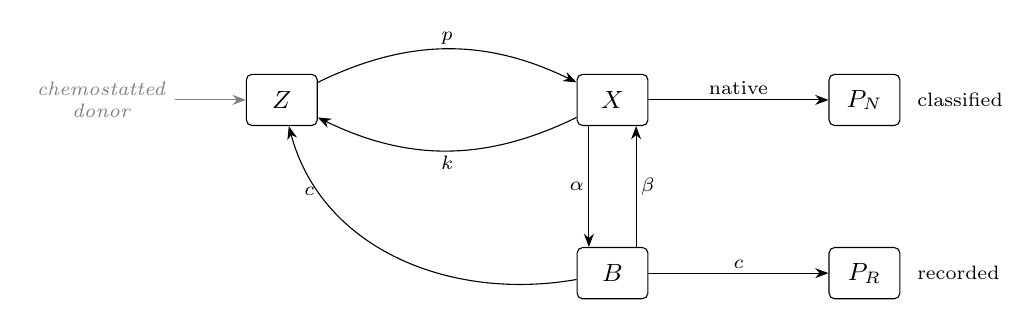
\begin{tikzpicture}[>=Stealth,x=1mm,y=1mm,
  sp/.style={draw,rounded corners=2pt,minimum height=6.5mm,minimum width=9mm,
             font=\small},
  lbl/.style={font=\scriptsize,inner sep=1.6pt},
  ext/.style={font=\scriptsize\itshape,gray}]
\node[sp] (Z) at (0,0) {$Z$};
\node[sp] (X) at (42,0) {$X$};
\node[sp] (B) at (42,-22) {$B$};
\node[sp] (PN) at (74,0) {$P_N$};
\node[sp] (PR) at (74,-22) {$P_R$};
\draw[->] (Z) to[bend left=26] node[lbl,above] {$p$} (X);
\draw[->] (X) to[bend left=26] node[lbl,below] {$k$} (Z);
\draw[->] (X) -- node[lbl,above] {native} (PN);
\draw[->] ([xshift=-3mm]X.south) -- node[lbl,left] {$\alpha$}
  ([xshift=-3mm]B.north);
\draw[->] ([xshift=3mm]B.north) -- node[lbl,right] {$\beta$}
  ([xshift=3mm]X.south);
\draw[->] (B) -- node[lbl,above] {$c$} (PR);
\draw[->] (B) to[out=190,in=285] node[lbl,left,pos=0.8] {$c$} (Z);
\node[ext,left=9mm of Z,align=center] (feed) {chemostatted\\donor};
\draw[->,gray] (feed) -- (Z);
\node[lbl,right=1.5mm of PN] {classified};
\node[lbl,right=1.5mm of PR] {recorded};
\end{tikzpicture}
\caption{The source \eqref{eq:reactions}. Association ($\alpha$) consumes free
reporter $R$; dissociation ($\beta$) and catalytic release ($c$) return it. The
reporter both consumes the reduced cofactor and, while the complex $B$
persists, withholds it from the regeneration channel: the release arrow returns
that cofactor to the \emph{oxidised} pool $Z$, not to $X$. The recorded
observable is the reporter product $P_R$; the quantity being classified is the
rate of native product $P_N$.}
\label{fig:scheme}
\end{figure}

With concentrations $x,z,b,q$ for $X,Z,B,P_R$, conserved totals
$x+z+b=C$ and $r+b=R_t$, and the abbreviations
\[
a:=p+k,\qquad h:=\beta+c,\qquad u:=\frac{\alpha R_t c}{h},
\]
mass action gives
\begin{equation}
\begin{aligned}
x'&=p\,(C-x-b)-kx-\alpha x\,(R_t-b)+\beta b,\\
b'&=\alpha x\,(R_t-b)-hb,\qquad
q'=cb,\qquad P_N'=kx .
\end{aligned}
\label{eq:source}
\end{equation}
All rates and totals are positive. The regeneration term acts on the
\emph{oxidised} pool $z=C-x-b$, not on $x$; this is what makes the complex a
store rather than a mere sink, and it is the point at which an
instantaneous-turnover idealisation loses information. Table~\ref{tab:symbols}
collects the notation.

\begin{table}[ht]
\centering\small
\begin{tabularx}{\textwidth}{llY}
\toprule
Symbol & Meaning & Role \\
\midrule
$x,z,b$ & free reduced, free oxidised, bound cofactor & state \\
$C=x+z+b$ & conserved total cofactor & invariant \\
$R_t=r+b$ & total active reporter & invariant \\
$p$ & effective regeneration coefficient, acting on $z$ & class parameter \\
$k$ & effective native-use coefficient, acting on $x$ & calibrated \\
$\alpha,\beta,c$ & association, dissociation, catalytic release & reporter \\
$a=p+k$, $h=\beta+c$ & relaxation rate, complex clearance rate & derived \\
$u=\alpha R_t c/h$ & effective reporter activity & derived, not primitive \\
$q$ & accumulated reporter product & recorded \\
$F=kpC/(p+k)$ & stationary reference native flux & classified \\
$\eta$ & relative preparation uncertainty & contract \\
$g,E$ & detector gain, additive error bound & contract \\
\bottomrule
\end{tabularx}
\caption{Notation. The effective activity $u$ is a derived combination of
$\alpha,R_t,\beta,c$, not an independent primitive: a design that fixes the four
primitives independently must check that the resulting $u$ lies in the admitted
interval.}
\label{tab:symbols}
\end{table}

\subsection{Matched preparation and reference}

Write $\xb:=pC/a$ for the reporter-free stationary free-pool level. The
preparation satisfies
\begin{equation}
b(0)=q(0)=0,\qquad x(0)=\xb(1+s),\quad |s|\le\eta<1,\qquad x(0)\le C,
\label{eq:prep}
\end{equation}
and the matched reporter-free reference starts from the same free cofactor in
the same environment, so that
\begin{equation}
x_0(t)=\xb\bigl(1+s\,e^{-at}\bigr),\qquad
F=\frac{kpC}{p+k}.
\label{eq:ref}
\end{equation}
The classified function is the stationary reference flux $F$. Disturbance,
however, is always measured against the \emph{actual} matched trajectory
$kx_0(t)$, never against an equilibrium substituted after the experiment has
begun. Define
\begin{equation}
e:=x_0-x,\qquad w:=e-b,\qquad
I(t):=\int_0^t b,\qquad D(t):=\int_0^t k e .
\label{eq:deficits}
\end{equation}
$D$ is the cumulative native-output deficit; $w$ is the deficit net of what is
currently in store. Outside the regime $c\ge k$ studied below, $D$ should be
read as a signed account until its sign has been established.

\subsection{Observation and intervention}

The endpoint record is
\begin{equation}
Y=g\,q(T)+\xi,\qquad |\xi|\le E,
\label{eq:record}
\end{equation}
with a calibrated positive gain $g$. The reporter product is assumed stable over
the recording interval and the detector linear on the admitted range. Reporter
turnovers are not identified with photon counts, and \eqref{eq:record} is a
deterministic envelope, not an error probability.

Acquisition uses a constant association coefficient on $[0,T]$. Afterwards the
experiment intervenes to stop \emph{new} binding, leaving existing complex to
dissociate or turn over. Two versions of this intervention appear below: the
ideal switch $\alpha\equiv0$ for $t>T$, and the physically weaker hypothesis
\begin{equation}
0\le\alpha(T+s)\le\alpha_0\,e^{-\gamma s},\qquad \gamma>0,
\label{eq:fade}
\end{equation}
where $\alpha_0$ is the acquisition value. In both cases the intervention must
not remove bound cofactor from the system: an operation that withdraws the
reporter together with its cargo changes the conservation law and invalidates
every account below. This is a physical contract, and Section~\ref{sec:physical}
returns to what would be required to meet it.

The binary decision of Section~\ref{sec:main} additionally assumes that the
specimen belongs to one of two separated parameter classes. Without that
promise a threshold alone certifies nothing, and Section~\ref{sec:outer}
supplies the continuous alternative.

% ===========================================================================
\section{Exact accounting of the native-output cost}
\label{sec:account}
% ===========================================================================

\subsection{Existence and the physical domain}

\begin{proposition}[Invariance and global solutions]\label{prop:domain}
Let $\alpha:[0,\infty)\to[0,\infty)$ be measurable and locally bounded. The set
\[
\dom:=\{(x,b): x\ge0,\ b\ge0,\ x+b\le C,\ b\le R_t\}
\]
is forward invariant for \eqref{eq:source}, and every solution starting in
$\dom$ exists and remains in $\dom$ for all $t\ge0$.
\end{proposition}

\begin{proof}
On each face of $\dom$ the vector field points inward. At $x=0$,
$x'=p(C-b)+\beta b\ge0$ because $C-b\ge0$ on $\dom$. At $b=0$,
$b'=\alpha xR_t\ge0$. At $b=R_t$, $b'=-hR_t<0$. At $z=C-x-b=0$,
$(x+b)'=pz-kx-cb=-(kx+cb)\le0$. The field is polynomial in the state with
locally bounded measurable coefficients, hence locally Lipschitz in the state
uniformly on compacts, so Carath\'eodory solutions exist, are unique, and cannot
leave the compact set $\dom$; boundedness rules out finite-time blow-up. The
piecewise intervention of Section~\ref{sec:source} joins two such solutions
continuously.
\end{proof}

\subsection{The finite-time account}

\begin{proposition}[Finite-time account]\label{prop:finite}
For matched preparation $e(0)=b(0)=0$ and any $t\ge0$,
\begin{equation}
e'=-ae+b'+(p+c)\,b,
\qquad
w'=-aw+(c-k)\,b,
\label{eq:deficit-ode}
\end{equation}
and consequently
\begin{equation}
a\,D(t)=k\bigl[(p+c)I(t)+b(t)-e(t)\bigr].
\label{eq:finite}
\end{equation}
\end{proposition}

\begin{proof}
Subtract the reference equation $x_0'=p(C-x_0)-kx_0$ from the first line of
\eqref{eq:source}. The association terms cancel against $b'$:
\[
e'=x_0'-x'=-p(x_0-x-b)-k(x_0-x)+\alpha x(R_t-b)-\beta b
=-ae+pb+\alpha x(R_t-b)-\beta b .
\]
Substituting $\alpha x(R_t-b)=b'+hb=b'+\beta b+cb$ gives the first identity in
\eqref{eq:deficit-ode}; subtracting $b'$ and using $w=e-b$ gives the second.
Integrating the first identity from $0$ to $t$ with $e(0)=b(0)=0$ yields
\eqref{eq:finite}.
\end{proof}

Identity \eqref{eq:finite} is exact and finite: it contains the terminal complex
$b(t)$ and the terminal free-pool deficit $e(t)$ explicitly. Omitting them
understates the eventual cost of a short acquisition, because a short window
leaves much of its cost in store.

\subsection{The complete-recovery cost is a schedule invariant}

The next statement is the central result. It requires no shut-off contract at
all: only that the reporter is eventually switched off in the weak sense that
the total association mass is finite.

\begin{theorem}[Schedule-invariant cost per reporter product]\label{thm:invariant}
Let $\alpha:[0,\infty)\to[0,\infty)$ be measurable and locally bounded, let the
preparation be matched as in \eqref{eq:prep}, and suppose the total association
mass is finite:
\begin{equation}
V_0:=\int_0^\infty \alpha(t)\,x(t)\bigl(R_t-b(t)\bigr)\dd t<\infty .
\label{eq:exposure}
\end{equation}
Then $b(t)\to0$ and $e(t)\to0$, the limits
$q_\infty=\lim_{t\to\infty}q(t)$ and $D_\infty=\lim_{t\to\infty}D(t)$ exist and
are finite, and
\begin{equation}
\boxed{\;
q_\infty=c\int_0^\infty b=\frac{c\,V_0}{h},
\qquad
D_\infty=\frac{k(p+c)}{ac}\,q_\infty
=\frac{k}{p+k}\Bigl(1+\frac pc\Bigr)q_\infty .\;}
\label{eq:invariant}
\end{equation}
In particular the complete-recovery native-output loss per unit of reporter
product depends only on $p$, $k$ and $c$; it is independent of $\beta$, of
$R_t$, of $C$, of the preparation offset $s$, and of the entire association
schedule.
\end{theorem}

\begin{proof}
Write $v(t):=\alpha(t)x(t)(R_t-b(t))\ge0$, so that $b'=v-hb$ and
$b(t)=\int_0^t e^{-h(t-\sigma)}v(\sigma)\dd\sigma$ since $b(0)=0$. Integrating
$b'=v-hb$ on $[0,t]$ gives $h\int_0^t b=\int_0^t v-b(t)\le V_0$, so
$\int_0^\infty b$ converges and $h\int_0^\infty b=V_0$ once we know
$b(t)\to0$. For that, fix $\varepsilon>0$ and choose $T_\varepsilon$ with
$\int_{T_\varepsilon}^\infty v<\varepsilon$; for $t>T_\varepsilon$,
\[
b(t)\le e^{-h(t-T_\varepsilon)}\int_0^{T_\varepsilon}v
+\int_{T_\varepsilon}^{t}v<\varepsilon+o(1),
\]
so $\limsup b\le\varepsilon$ for every $\varepsilon$, i.e.\ $b(t)\to0$.
Since $q'=cb\ge0$ and $\int_0^\infty b<\infty$, the limit $q_\infty=c\int_0^\infty b
=cV_0/h$ exists.

Next, $w'=-aw+(c-k)b$ with $w(0)=0$ gives
$w(t)=\int_0^t e^{-a(t-\sigma)}(c-k)b(\sigma)\dd\sigma$, so $|w|$ is bounded by
$|c-k|$ times the convolution of an integrable function with an exponential
kernel; hence $w\in L^1(0,\infty)$ with
$a\int_0^\infty w=(c-k)\int_0^\infty b$, and $w(t)\to0$ by the same argument
used for $b$. Therefore $e=w+b\to0$ and $e\in L^1(0,\infty)$, so
$D_\infty=k\int_0^\infty e$ is finite. Letting $t\to\infty$ in \eqref{eq:finite}
and using $e(t),b(t)\to0$ gives $aD_\infty=k(p+c)I_\infty$ with
$I_\infty=q_\infty/c$, which is \eqref{eq:invariant}.
\end{proof}

\begin{remark}
$D_\infty$ is a convergent integral of a \emph{difference} of fluxes. It is
never obtained by subtracting two divergent cumulative production totals, and the
proof does not require the reference and the measured trajectory to be compared
at any particular finite time.
\end{remark}

\subsection{What the factor means, and what evades it}
\label{sec:meaning}

In the instantaneous-turnover idealisation, in which the complex is eliminated
and the reporter acts as a first-order sink of strength $u$, the same
computation gives $D_\infty=kq_\infty/a$. The explicit complex multiplies this by
\begin{equation}
1+\frac pc .
\label{eq:factor}
\end{equation}
Table~\ref{tab:factor} evaluates it at $p=1$.

\begin{table}[ht]
\centering\small
\begin{tabular}{lcccc}
\toprule
catalytic release $c$ & $0.2$ & $1$ & $5$ & $20$\\
\midrule
storage factor $1+p/c$ at $p=1$ & $6$ & $2$ & $1.2$ & $1.05$\\
\bottomrule
\end{tabular}
\caption{The complete-recovery cost per reporter product, relative to the
instantaneous-turnover prediction, for four catalytic release coefficients at
equal effective activity $u$ and equal final reporter product.}
\label{tab:factor}
\end{table}

Two quantities are easy to conflate here, and the distinction is the whole
content of \eqref{eq:factor}.
\begin{itemize}
\item The \emph{mean residence of one binding episode} is $1/h=1/(\beta+c)$.
Dissociation shortens it.
\item The \emph{accumulated bound occupancy per successful reporter product} is
$1/c$, because $q_\infty=c\,I_\infty$. Dissociation does not shorten it: a
dissociated complex returns its cofactor but produces nothing, so the reporter
must bind again.
\end{itemize}
This is why $\beta$ disappears from \eqref{eq:invariant} while remaining
important for transients, and why increasing $\beta$ at fixed $u$ and fixed
final product is not a substitute for increasing $c$.

Theorem~\ref{thm:invariant} also delimits the claim. The factor is a property of
\emph{this} source at fixed final reporter product. It is evaded by changing the
chemistry, not the protocol: a reporter that does not consume the cofactor, one
that returns it in the reduced form, an externally replenished pool, or simply a
larger $c$. There is no universal lower bound here for every measurement
technology, and none is claimed.

% ===========================================================================
\section{Uniform envelopes and a design criterion}
\label{sec:envelopes}
% ===========================================================================

Throughout this section the reporter is calibrated in the regime
\begin{equation}
c\ge k,
\label{eq:regime}
\end{equation}
which says the reporter releases its cargo at least as fast as the native
reaction consumes free cofactor. This is the regime in which the deficit account
is signed, and it is the regime the design targets.

\subsection{Preservation}

\begin{proposition}[Uniform preservation]\label{prop:pres}
Assume \eqref{eq:prep}, \eqref{eq:regime} and $0\le\alpha(t)\le\alpha_0$ for all
$t$, with $u_0:=\alpha_0R_tc/h$. Then $w\ge0$, hence $e\ge b\ge0$ and
$x\le x_0$, and for all $t\ge0$
\begin{equation}
0\le b(t)\le\frac{u_0(1+\eta)\xb}{c},
\qquad
0\le e(t)\le(1+\eta)\,\xb\,\frac{u_0}{a}\Bigl(1+\frac pc\Bigr),
\qquad
\frac{e(t)}{x_0(t)}\le\frac{1+\eta}{1-\eta}\cdot\frac{u_0}{a}\Bigl(1+\frac pc\Bigr).
\label{eq:pres}
\end{equation}
\end{proposition}

\begin{proof}
By \eqref{eq:deficit-ode}, $w'=-aw+(c-k)b$ with $w(0)=0$, so variation of
constants gives $w(t)=\int_0^te^{-a(t-\sigma)}(c-k)b(\sigma)\dd\sigma\ge0$,
using $b\ge0$ from Proposition~\ref{prop:domain} and $c\ge k$. Hence
$e=w+b\ge b\ge0$ and $x=x_0-e\le x_0\le(1+\eta)\xb$.

Because $R_t-b\le R_t$ and $x\le(1+\eta)\xb$,
\[
b'\le\alpha_0R_t(1+\eta)\xb-hb ,
\]
and comparison with the scalar linear equation from $b(0)=0$ gives
$b\le\alpha_0R_t(1+\eta)\xb/h=u_0(1+\eta)\xb/c$, which is the first bound.
Feeding it into the representation of $w$ gives
$w\le(c-k)u_0(1+\eta)\xb/(ca)$, so
\[
e=w+b\le\frac{u_0(1+\eta)\xb}{c}\Bigl(1+\frac{c-k}{a}\Bigr)
=(1+\eta)\xb\,\frac{u_0}{a}\Bigl(1+\frac{p}{c}\Bigr),
\]
where the last step uses $a+c-k=p+c$. Dividing by $x_0\ge(1-\eta)\xb>0$ gives
the third bound. Every comparison above is an integration of a differential
inequality against its positive integrating factor; no extremum of a nonlinear
trajectory at a corner of a parameter box is assumed anywhere.
\end{proof}

\begin{remark}
The hypothesis is $\alpha(t)\le\alpha_0$, not $\alpha\equiv\alpha_0$ on $[0,T]$
followed by zero. Proposition~\ref{prop:pres} therefore covers acquisition, an
ideal switch, and any fading switch \eqref{eq:fade} whose amplitude does not
exceed the acquisition value. Preservation is never the difficult half of the
recovery analysis.
\end{remark}

\subsection{Signal}

\begin{proposition}[Lower and upper signal envelopes]\label{prop:signal}
Let $B_0$ be any uniform upper bound for $u(1+p/c)/a$ over the admitted
parameters and set $m:=1-\eta-(1+\eta)B_0$. If $m>0$ then $x\ge m\xb$
throughout, and for constant association on $[0,T]$ with $T\ge1/h$,
\begin{equation}
\frac{u\,m\,\xb}{1+u\,m\,\xb/(cR_t)}\Bigl(T-\frac1h\Bigr)
\;\le\; q(T)\;\le\; u(1+\eta)\,\xb\,T .
\label{eq:signal}
\end{equation}
\end{proposition}

\begin{proof}
From \eqref{eq:pres}, $x=x_0-e\ge(1-\eta)\xb-(1+\eta)\xb B_0=m\xb$. Using
$x\ge m\xb$ and $R_t-b\ge0$,
\[
b'\ge\alpha m\xb\,(R_t-b)-hb=\alpha R_t m\xb-\lambda b,
\qquad \lambda:=h+\alpha m\xb\ \ge h .
\]
Comparison from $b(0)=0$ gives $b(t)\ge(\alpha R_tm\xb/\lambda)(1-e^{-\lambda t})$,
hence
\[
q(T)=c\int_0^Tb
\ \ge\ \frac{c\,\alpha R_t m\xb}{\lambda}\Bigl(T-\frac{1-e^{-\lambda T}}{\lambda}\Bigr)
\ \ge\ \frac{c\,\alpha R_t m\xb}{\lambda}\Bigl(T-\frac1h\Bigr).
\]
Finally $c\alpha R_t/\lambda=u/(1+\alpha m\xb/h)$ and $\alpha/h=u/(cR_t)$ give
the stated left-hand side. The right-hand side is $c$ times the uniform bound on
$b$ from \eqref{eq:pres} integrated over $[0,T]$.
\end{proof}

\subsection{The design criterion}

Proposition~\ref{prop:pres} and Proposition~\ref{prop:signal} combine into a
criterion stated entirely in terms of interval endpoints. Write $\square_-$ and
$\square_+$ for the smallest and largest admitted value of a quantity, and let
$\xb^{\mathrm{lo}}_+$ and $\xb^{\mathrm{hi}}_-$ denote the largest reference
level attainable in the low class and the smallest attainable in the high class;
since $\xb=pC/(p+k)$ increases in $p$ and $C$ and decreases in $k$, these are
attained at interval endpoints.

\begin{theorem}[Design criterion]\label{thm:criterion}
Assume \eqref{eq:prep}, \eqref{eq:regime}, $c_-\ge k_+$, and put
\[
B_0:=\frac{u_+}{a_-}\Bigl(1+\frac{p_+}{c_-}\Bigr),\qquad
m:=1-\eta-(1+\eta)B_0,\qquad
\sigma:=\frac{u_+C_+}{c_-R_-} .
\]
Let $\delta$ be the prescribed relative disturbance tolerance.
\begin{enumerate}
\item[\textup{(i)}] \textup{(Preservation.)} If
$\frac{1+\eta}{1-\eta}B_0\le\delta$ and $m>0$, then for every admitted source and
preparation, and at every time during acquisition and any subsequent
intervention with $\alpha\le\alpha_0$,
\[
0\le\frac{kx_0(t)-kx(t)}{kx_0(t)}\le\delta .
\]
\item[\textup{(ii)}] \textup{(Discrimination.)} If moreover $T\ge1/h_-$ and
\begin{equation}
\underbrace{g_-u_-\,m\,\xb^{\mathrm{hi}}_-\,\frac{T-1/h_-}{1+\sigma}}_{=:L(T)}
\;-\;
\underbrace{g_+u_+(1+\eta)\,\xb^{\mathrm{lo}}_+\,T}_{=:U(T)}
\;>\;2E ,
\label{eq:criterion}
\end{equation}
then every record compatible with the low class satisfies $Y\le U(T)+E$, every
record compatible with the high class satisfies $Y\ge L(T)-E$, and the threshold
$\theta=\bigl(U(T)+L(T)\bigr)/2$ classifies every admitted specimen correctly.
\end{enumerate}
\end{theorem}

\begin{proof}
Part (i) is the third bound of \eqref{eq:pres}, evaluated at the interval
endpoints that maximise it: $u/a\le u_+/a_-$ and $p/c\le p_+/c_-$. Part (ii)
applies \eqref{eq:signal}, multiplies by the gain bounds and adds the detector
envelope \eqref{eq:record}. The monotonicity of $\xb$ in $p$, $C$, $k$ has the
stated derivatives $Ck/(p+k)^2>0$, $p/(p+k)>0$ and $-pC/(p+k)^2<0$, so its
extrema over the box are attained at endpoints, and the saturation denominator
is bounded by $1+\sigma$ using $m\le1$ and $\xb\le C$. Under
\eqref{eq:criterion} the two closed record intervals $[\,\cdot\,,U(T)+E]$ and
$[L(T)-E,\,\cdot\,]$ are disjoint and $\theta$ lies strictly between them.
\end{proof}

Theorem~\ref{thm:criterion} is the useful form for a designer: it says which
quantities must be calibrated, and it exposes the trade-off. Larger $T$ helps
discrimination linearly and does not affect preservation; larger $u$ helps
discrimination but enters preservation directly; smaller $c$ hurts both, through
$B_0$ and through $\sigma$.

% ===========================================================================
\section{A robust finite-time protocol}
\label{sec:main}
% ===========================================================================

\begin{theorem}[Robust joint protocol]\label{thm:main}
Consider \eqref{eq:source}--\eqref{eq:ref} with the dimensionless intervals
\begin{gather*}
p\in[0.95,1.05]\ \text{(low class)},\qquad p\in[1.95,2.05]\ \text{(high class)},\\
k\in[0.98,1.02],\quad C\in[0.99,1.01],\quad R_t\in[0.99,1.01],\quad \eta=0.01,\\
u=\frac{\alpha R_tc}{\beta+c}\in[0.079,0.081],\quad c\in[20,25],\quad
\beta\in[1,2],\quad g\in[0.98,1.02],\quad E=0.01,
\end{gather*}
acquisition $T=8$ and recovery $\tau=5$. Then, for every admitted source and
preparation, at every time during acquisition and recovery,
\begin{equation}
0\le\frac{kx_0(t)-kx(t)}{kx_0(t)}\le\frac{400869}{8492000}
=0.047205\ldots<0.0473<0.05,
\label{eq:main-pres}
\end{equation}
and in absolute terms $e(t)<0.032$ and $b(t)<0.0028$ concentration units. The
low class has stationary native flux below $0.523$ and the high class above
$0.645$. With
\[
\begin{aligned}
U(T)&=\frac{102}{100}\cdot\frac{81}{1000}\cdot\frac{101}{100}\cdot
\frac{(105/100)(101/100)}{203/100}\,T,\\[2pt]
L(T)&=\frac{98}{100}\cdot\frac{79}{1000}\cdot\frac{94}{100}\cdot
\frac{(195/100)(99/100)}{297/100}\cdot\frac{T-1/21}{1005/1000},
\end{aligned}
\]
every compatible low record is at most $U(8)+0.01$ and every compatible high
record is at least $L(8)-0.01$, where
\[
U(8)=\frac{126420993}{362500000}=0.34874756\ldots,\qquad
L(8)=\frac{56426461}{150750000}=0.37430488\ldots,
\]
\[
L(8)-U(8)-0.02=\frac{1214759671}{218587500000}=0.00555731\ldots>0.005 .
\]
The threshold $\theta=(U(8)+L(8))/2=0.36152622\ldots$ therefore separates the
two classes strictly, with per-class slack exceeding $0.0027$. After the
recovery period the outstanding native-output loss is below $3\cdot10^{-6}$
concentration units \textup{(}Theorem~\ref{thm:ideal}\textup{)}.
\end{theorem}

\begin{proof}
On this box $a\ge1.93$, $a\le3.07$, $h\ge21$, $h\le27$, $p\le2.05$ and
$c\ge20\ge1.02\ge k$, so \eqref{eq:regime} holds. Take
\[
B_0=\frac{0.081\,(1+2.05/20)}{1.93}=\frac{35721}{772000},
\]
which dominates $u(1+p/c)/a$ over the box. Exact rational arithmetic gives
\[
\frac{1.01}{0.99}B_0=\frac{400869}{8492000}<0.0473,
\qquad
m=1-0.01-1.01\,B_0=\frac{72820179}{77200000}>0.94,
\]
which is \eqref{eq:main-pres} and the free-pool floor. For the absolute bounds,
$\xb=pC/(p+k)\le(2.05)(1.01)/(2.05+0.98)=41/60$, so by \eqref{eq:pres}
$e\le1.01\cdot(41/60)\cdot B_0<0.032$ and
$b\le0.081\cdot1.01\cdot(41/60)/20<0.0028$.

For discrimination, $\sigma=0.081\cdot1.01/(20\cdot0.99)=909/220000<0.005$, so
the saturation denominator is at most $1.005$, and $T=8\ge1/21$. The extreme
reference levels are $\xb^{\mathrm{lo}}_+=(1.05)(1.01)/2.03$ and
$\xb^{\mathrm{hi}}_-=(1.95)(0.99)/2.97$. Substituting these, together with
$m\ge0.94$, into Theorem~\ref{thm:criterion}(ii) gives exactly the displayed
$U$ and $L$; the displayed rational values of $U(8)$, $L(8)$, their separation
and the threshold are exact. The class flux bounds follow because
$F=kpC/(p+k)$ increases in each of $p,k,C$, so
$F\le(1.02)(1.05)(1.01)/2.07<0.523$ in the low class and
$F\ge(0.98)(1.95)(0.99)/2.93>0.645$ in the high class.
\end{proof}

\begin{remark}[What the theorem is not]
The region is a \emph{sufficient inner} region. The inequalities are strict, so
the admitted design has genuine slack; but failure of the same rounded
certificate at a shorter acquisition is not an impossibility proof. With the
rounded constants above, the margin $L(T)-U(T)-0.02$ equals $-0.00139$ at
$T=6$, $+0.00208$ at $T=7$ and $+0.00556$ at $T=8$: the printed certificate
first closes at $T=7$. Nothing here classifies all protocols, and no optimality
is claimed.
\end{remark}

\begin{remark}[Two contracts, not one]
The rounded envelopes of Theorem~\ref{thm:main} and the unrounded envelopes of
Theorem~\ref{thm:criterion} are both valid, but they define different thresholds.
An observation threshold from one contract must never be combined with signal
envelopes from the other.
\end{remark}

% ===========================================================================
\section{Finite recovery, with and without an ideal switch}
\label{sec:recovery}
% ===========================================================================

\subsection{The outstanding-loss functional}

\begin{proposition}[Remainder identity]\label{prop:remainder}
Suppose the hypotheses of Theorem~\ref{thm:invariant} hold, and let $t\ge0$.
Write $V(t):=\int_t^\infty v$ for the remaining association mass. Then the
outstanding native-output loss $\Rem(t):=D_\infty-D(t)=k\int_t^\infty e$
satisfies
\begin{equation}
\Rem(t)=\frac ka\Bigl[w(t)+\frac{p+c}{h}\bigl(b(t)+V(t)\bigr)\Bigr]
=\frac ka\Bigl[e(t)+\frac{p-\beta}{h}\,b(t)+\frac{p+c}{h}V(t)\Bigr].
\label{eq:remainder}
\end{equation}
In the regime $c\ge k$ every term of the first expression is nonnegative.
\end{proposition}

\begin{proof}
Integrating $e'=-ae+b'+(p+c)b$ on $[t,\infty)$ and using $e,b\to0$ gives
$a\int_t^\infty e=e(t)-b(t)+(p+c)\int_t^\infty b=w(t)+(p+c)\int_t^\infty b$.
Integrating $b'=v-hb$ on $[t,\infty)$ gives
$h\int_t^\infty b=b(t)+V(t)$. Multiplying by $k$ gives the first form; the
second follows from $w=e-b$ and $h=\beta+c$, since
$-b+(p+c)b/h=(p-\beta)b/h$.
\end{proof}

The first form of \eqref{eq:remainder} is the one to use in bounds: it is a sum
of nonnegative terms, so upper bounds may be substituted term by term without
worrying about the sign of $p-\beta$.

\subsection{Ideal switch}

\begin{theorem}[Ideal-switch recovery]\label{thm:ideal}
Under the hypotheses of Theorem~\ref{thm:main}, with $\alpha\equiv0$ for $t>T$,
\[
\Rem(T+\tau)\;\le\;\frac{k_+}{a_-}\Bigl[
\Bigl(e_*+\frac{d_*\,b_*}{h_--a_-}\Bigr)e^{-a_-\tau}
+\frac{(p+c)_+}{h_-}\,b_*\,e^{-h_-\tau}\Bigr],
\]
where $e_*=0.032$, $b_*=0.0028$, $d_*=c_+-k_-=24.02$, $a_-=1.93$, $h_-=21$ and
$(p+c)_+=27.05$. At $\tau=5$ this is below $1.5\cdot10^{-6}$, hence below
$3\cdot10^{-6}$, concentration units.
\end{theorem}

\begin{proof}
After the switch $V\equiv0$ and $b(T+s)=b(T)e^{-hs}\le b_*e^{-h_-s}$. For $w$,
$w'=-aw+(c-k)b$ gives
\[
w(T+s)=w(T)e^{-as}+\int_0^s e^{-a(s-\sigma)}(c-k)\,b(T+\sigma)\dd\sigma
\le e_*e^{-a_-s}+d_*b_*\int_0^se^{-a_-(s-\sigma)}e^{-h_-\sigma}\dd\sigma,
\]
where we used $w(T)\le e(T)\le e_*$, $a\ge a_-$ for the kernel and $h\ge h_-$
for the forcing. The remaining integral equals
$(e^{-a_-s}-e^{-h_-s})/(h_--a_-)\le e^{-a_-s}/(h_--a_-)$. Substituting into
the first form of \eqref{eq:remainder} and using $k/a\le k_+/a_-$ and
$(p+c)/h\le(p+c)_+/h_-$ gives the display. At $\tau=5$, the degree-$16$ Taylor
partial sum of $e^{9.65}$ exceeds $15208$, so $e^{-9.65}<1/14000$, and the
resulting rational expression evaluates to less than $1.21\cdot10^{-6}$; using
the single crude bound $e^{-105}\le e^{-9.65}<1/14000$ for both exponentials
still gives less than $1.48\cdot10^{-6}$.
\end{proof}

\subsection{Fading switch}

The ideal switch is the mathematically convenient intervention, not the
physically available one. We now assume only \eqref{eq:fade}. Write
\[
A_*:=\sup\alpha_0CR_t=\frac{u_+h_+C_+}{c_-}=0.1104435,
\]
which bounds the association flux amplitude immediately after acquisition,
because $v=\alpha x(R_t-b)\le\alpha_0e^{-\gamma s}CR_t$ and
$\alpha_0=u h/(R_tc)$.

\begin{lemma}[Two-rate convolution bound]\label{lem:conv}
Let $r,\rho>0$ and let $\nu>0$ satisfy $\nu\le r$ and $\nu<\rho$. Then for all
$s\ge0$,
\[
\int_0^s e^{-r(s-\sigma)}e^{-\rho\sigma}\dd\sigma\;\le\;\frac{e^{-\nu s}}{\rho-\nu},
\qquad
\int_0^s e^{-r(s-\sigma)}\sigma\,e^{-\rho\sigma}\dd\sigma
\;\le\;\frac{e^{-\nu s}}{(\rho-\nu)^2}.
\]
The same bounds hold with the roles of $r$ and $\rho$ interchanged.
\end{lemma}

\begin{proof}
Since $\nu\le r$ we may dominate the kernel, $e^{-r(s-\sigma)}\le
e^{-\nu(s-\sigma)}$ for $\sigma\le s$. Then
$\int_0^se^{-\nu(s-\sigma)}e^{-\rho\sigma}\dd\sigma
=e^{-\nu s}\int_0^se^{-(\rho-\nu)\sigma}\dd\sigma\le e^{-\nu s}/(\rho-\nu)$,
and similarly $\int_0^s\sigma e^{-(\rho-\nu)\sigma}\dd\sigma\le(\rho-\nu)^{-2}$.
The integrand is symmetric under $(r,\sigma)\leftrightarrow(\rho,s-\sigma)$,
which gives the interchanged form.
\end{proof}

\begin{theorem}[Fading-switch recovery]\label{thm:fade}
Assume the box of Theorem~\ref{thm:main} and \eqref{eq:fade}. Choose rates
$\nu_1,\nu_0>0$ admissible for Lemma~\ref{lem:conv} in the sense that
$\nu_1$ is admissible for the pair $(h_-,\gamma)$ with denominator $d_1$, and
$\nu_0$ is admissible for the pair $(a_-,\nu_1)$ with denominator $d_0$. Put
\[
\beta_*:=b_*+\frac{A_*}{d_1},\qquad
B_*:=e_*+\frac{d_*\,\beta_*}{d_0}.
\]
Then for all $s\ge0$,
\[
b(T+s)\le\beta_*e^{-\nu_1s},\qquad
w(T+s)\le B_*e^{-\nu_0s},\qquad
V(T+s)\le\frac{A_*}{\gamma}e^{-\gamma s},
\]
and consequently
\begin{equation}
0\;\le\;\Rem(T+s)\;\le\;\frac{k_+}{a_-}\Bigl[
B_*e^{-\nu_0s}
+\frac{(p+c)_+}{h_-}\Bigl(\beta_*e^{-\nu_1s}+\frac{A_*}{\gamma}e^{-\gamma s}\Bigr)
\Bigr].
\label{eq:fade-bound}
\end{equation}
Moreover the classifier of Theorem~\ref{thm:main} and the preservation bound
\eqref{eq:main-pres} are unaffected: the record is taken at $T$, and
Proposition~\ref{prop:pres} applies verbatim because $\alpha(T+s)\le\alpha_0$.
\end{theorem}

\begin{proof}
From $b'=v-hb$ and $b(T+s)\le b(T)e^{-hs}+\int_0^se^{-h(s-\sigma)}v(T+\sigma)
\dd\sigma$, with $b(T)\le b_*$, $h\ge h_-\ge\nu_1$ and $v(T+\sigma)\le
A_*e^{-\gamma\sigma}$, Lemma~\ref{lem:conv} gives
$b(T+s)\le b_*e^{-\nu_1s}+A_*e^{-\nu_1s}/d_1=\beta_*e^{-\nu_1s}$. Feeding this
into $w(T+s)\le w(T)e^{-as}+d_*\int_0^se^{-a(s-\sigma)}b(T+\sigma)\dd\sigma$
with $w(T)\le e_*$ and $a\ge a_-\ge\nu_0$, and applying Lemma~\ref{lem:conv}
again with the pair $(a_-,\nu_1)$, gives $w(T+s)\le B_*e^{-\nu_0s}$. The tail
mass obeys $V(T+s)\le\int_s^\infty A_*e^{-\gamma\sigma}\dd\sigma
=A_*e^{-\gamma s}/\gamma$, which is finite, so \eqref{eq:exposure} holds and
Proposition~\ref{prop:remainder} applies; substituting the three bounds into the
first, termwise nonnegative, form of \eqref{eq:remainder} gives
\eqref{eq:fade-bound}.
\end{proof}

\begin{corollary}[Five recovery units suffice for a fast fading switch]
\label{cor:fast-fade}
If $\gamma\ge21$, then taking $\nu_1=12$ and $\nu_0=1.93$ in
Theorem~\ref{thm:fade} gives $d_1=9$, $d_0=10.07$,
$\beta_*=0.0150667$ and $B_*=0.0678749$, and the outstanding loss at $\tau=5$
is below $2.4\cdot10^{-6}$, and below $4\cdot10^{-6}$ if all three exponentials
are crudely replaced by $e^{-9.65}<1/14000$. The original ideal-switch deadline
of five recovery units is therefore retained.
\end{corollary}

Table~\ref{tab:deadline} and Figure~\ref{fig:deadline} instantiate
Theorem~\ref{thm:fade} across decay rates, giving in each case the smallest
recovery time, to one decimal place, for which \eqref{eq:fade-bound} certifies an
outstanding loss below $3\cdot10^{-6}$. The deadline degrades gracefully: a
switch ten times slower than the complex-clearance rate costs roughly a
doubling of the recovery wait, not a loss of the guarantee.

\begin{table}[ht]
\centering\small
\begin{tabular}{ccccc}
\toprule
decay rate $\gamma$ & $\nu_0$ & $\nu_1$ & certified $\tau$ &
bound on $\Rem(T+\tau)$\\
\midrule
\recoveryrows
\bottomrule
\end{tabular}
\caption{Certified recovery deadlines from Theorem~\ref{thm:fade}, for the
parameter box of Theorem~\ref{thm:main} and target $3\cdot10^{-6}$. Each row is
verified in exact rational arithmetic, with every exponential replaced by a
rational upper bound obtained from a truncated exponential series; each listed
$\tau$ also fails the same test at $\tau-0.1$, so the tabulated values are tight
for this bound to one decimal place.}
\label{tab:deadline}
\end{table}

\begin{figure}[ht]
\centering
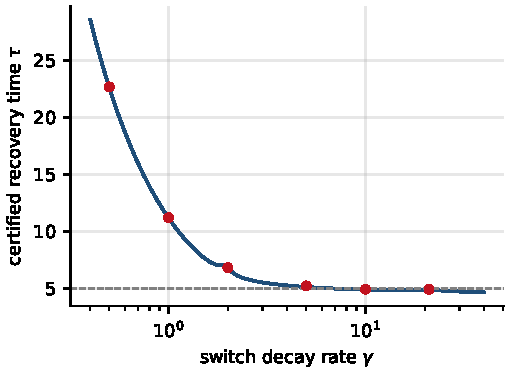
\includegraphics[width=0.52\linewidth]{figures/deadline.pdf}
\caption{The certified recovery time of Theorem~\ref{thm:fade} against the
switch decay rate $\gamma$, optimised over the admissible certified rates
$\nu_0,\nu_1$. Points mark the tabulated rows; the dashed line is the
five-unit deadline of Theorem~\ref{thm:main}. The curve flattens once $\gamma$
exceeds the relaxation rate $a$, because the remainder is then limited by the
cofactor pool's own relaxation rather than by the switch.}
\label{fig:deadline}
\end{figure}

\subsection{A small remainder is not no additional cost}

Theorem~\ref{thm:fade} bounds what is still \emph{outstanding} after the
recovery wait. It does not say that a fading switch is as cheap as an ideal one.

\begin{proposition}[Additional complete loss]\label{prop:extra}
Under \eqref{eq:fade}, the additional complete-recovery reporter product and
native-output loss caused by residual binding, relative to an ideal switch from
the same acquisition-end state, satisfy
\[
0\le\Delta q_\infty=\frac{c}{h}\int_T^\infty v\le\frac{cA_*}{h\gamma},
\qquad
0\le\Delta D_\infty=\frac ka\Bigl(1+\frac pc\Bigr)\Delta q_\infty
\le\frac ka\Bigl(1+\frac pc\Bigr)\frac{uC}{\gamma}.
\]
On the box of Theorem~\ref{thm:main} the right-hand bound is $0.002270$ at
$\gamma=21$ and $0.04767$ at $\gamma=1$.
\end{proposition}

\begin{proof}
Both statements are Theorem~\ref{thm:invariant} applied to the two schedules
that agree on $[0,T]$, together with $\int_T^\infty v\le A_*/\gamma$ and
$\alpha_0CR_t=uhC/c$, so that $cA_*/(h\gamma)$ simplifies to $uC/\gamma$ before
the cost factor is applied.
\end{proof}

At $\gamma=21$ the extra complete loss bound, $0.0023$, is three orders of
magnitude larger than the outstanding remainder, $2.4\cdot10^{-6}$. The two
numbers answer different questions: the remainder says the experiment may stop
waiting, the extra loss says what the imperfect switch cost. Numerically, at the
nominal parameters of Section~\ref{sec:numerics}, the realised extra complete
loss is $0.00096$ at $\gamma=21$, $0.00405$ at $\gamma=5$ and $0.02041$ at
$\gamma=1$, all within the proposition's bounds.

% ===========================================================================
\section{Continuous bounded-error inference}
\label{sec:outer}
% ===========================================================================

Theorem~\ref{thm:main} answers a binary question and needs a binary promise. The
same envelopes answer a continuous question with no extra assumption, by set
inversion \citep{jaulin1993}.

Admit $p$ anywhere in $[0.95,2.05]$, keeping every other interval as before. The
loading and free-pool bounds are unchanged, because their proof already used the
enclosing range. Writing the $p$-dependence of $\xb$ explicitly, the envelopes of
Theorem~\ref{thm:criterion} become
\begin{equation}
L_p=A_L\,\frac{p}{p+k_+},\qquad
U_p=A_U\,\frac{p}{p+k_-},
\label{eq:envelopes-p}
\end{equation}
with, at $T=8$,
\[
A_L=\frac{0.98\cdot0.079\cdot0.94\cdot0.99}{1.005}\Bigl(8-\frac1{21}\Bigr)
=\frac{47745467}{83750000}=0.5700951\ldots,
\]
\[
A_U=1.02\cdot0.081\cdot1.01^2\cdot8=\frac{42140331}{62500000}=0.6742453 .
\]

\begin{proposition}[Outer set and function interval]\label{prop:outer}
For a record $y$ satisfying the contract \eqref{eq:record}, define
\begin{equation}
\mathcal P(y):=\bigl\{p\in[0.95,2.05]:\ L_p\le y+E\ \text{and}\ U_p\ge y-E\bigr\}.
\label{eq:outer}
\end{equation}
Then the true $p$ lies in $\mathcal P(y)$. Both envelopes in
\eqref{eq:envelopes-p} are strictly increasing in $p$, so whenever
$0<y-E<A_U$ and $0\le y+E<A_L$ the set is the interval
$[p_-,p_+]\cap[0.95,2.05]$ with
\begin{equation}
p_-=\frac{k_-\,(y-E)}{A_U-y+E},\qquad
p_+=\frac{k_+\,(y+E)}{A_L-y-E}.
\label{eq:inversion}
\end{equation}
Because $F=kpC/(p+k)$ is increasing in each of $p,k,C$, the classified function
obeys
\begin{equation}
\frac{k_-C_-\,p_-}{p_-+k_-}\;\le\;F\;\le\;\frac{k_+C_+\,p_+}{p_++k_+} .
\label{eq:flux-interval}
\end{equation}
\end{proposition}

\begin{proof}
Membership is immediate: $g\,q(T)\in[L_p,U_p]$ and $|Y-gq(T)|\le E$. For the
inversion, $L_p\le y+E$ reads $A_Lp\le(y+E)(p+k_+)$, i.e.\
$p\,(A_L-y-E)\le k_+(y+E)$, which gives the upper endpoint when
$A_L>y+E$; the lower endpoint is the same computation applied to $U_p\ge y-E$.
Outside those ranges the defining inequalities in \eqref{eq:outer} are used
directly: a nonpositive lower requirement imposes no lower constraint, and a
record at or beyond the upper asymptote makes the set empty.
\end{proof}

\begin{remark}[Outer, not identified]
$\mathcal P(y)$ is an \emph{outer} enclosure. Because $L_p$ and $U_p$ are
sufficient envelopes rather than the exact attainable range of $gq(T)$, the set
may contain values of $p$ that no admitted source actually realises. An empty
$\mathcal P(y)$ therefore certifies incompatibility with the declared contract;
a nonempty $\mathcal P(y)$ does not certify that a compatible source exists.
\end{remark}

\begin{example}\label{ex:outer}
Two records, and the intervals they support:
\begin{center}\small
\begin{tabular}{ccc}
\toprule
record $y$ & outer set for $p$ & outer set for $F$\\
\midrule
$0.30549$ & $[0.9500,\,1.2639]$ & $[0.47756,\,0.57011]$\\
$0.41151$ & $[1.4427,\,2.0500]$ & $[0.57775,\,0.68792]$\\
\bottomrule
\end{tabular}
\end{center}
The first record excludes the high class, the second excludes the low class, and
neither needs the binary promise to do so. The intervals are wider than the
binary conclusions of Theorem~\ref{thm:main}, which is the appropriate price for
the weaker premise. A record at the binary threshold $\theta=0.36153$ yields the
outer set $p\in[1.0675,1.9084]$, which meets \emph{neither} promised class: this
is exactly what strict separation means, expressed in the continuous contract.
\end{example}

\begin{figure}[ht]
\centering
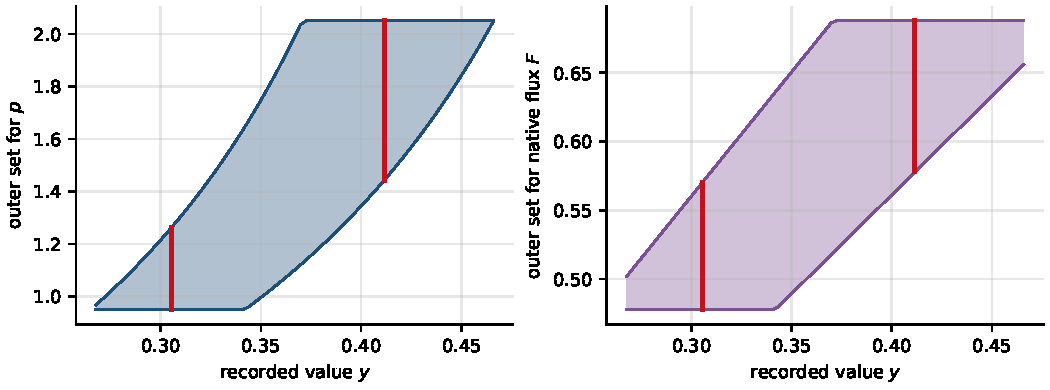
\includegraphics[width=\linewidth]{figures/inference.pdf}
\caption{Outer sets from Proposition~\ref{prop:outer} as a function of the
record $y$: left, for the regeneration capacity $p$; right, for the classified
stationary native flux $F$. Red segments mark the two records of
Example~\ref{ex:outer}. The sets flatten against the admitted range
$[0.95,2.05]$ at both ends, where the prior physical interval, not the record,
is binding. Records outside $[0.2650,0.4661]$ are incompatible with the
declared contract at every admitted $p$, and the plotted band stops there. A
functional threshold may be decided whenever the whole interval lies on one
side of it; otherwise the correct report is \emph{unresolved}.}
\label{fig:inference}
\end{figure}

A decision rule built on \eqref{eq:flux-interval} needs no point estimate: report
the functional verdict when the entire interval lies on one side of the
biological threshold, and report \emph{unresolved} otherwise. To upgrade such an
interval to a frequentist confidence statement one would have to supply a
calibration event with a stated coverage probability and prove the deterministic
implication on that event; to claim posterior contraction one would need a
stochastic observation model, an identifiable parameter class and an asymptotic
regime. Section~\ref{sec:alias} shows why the identifiability requirement is not
a formality.

% ===========================================================================
\section{Beyond linear native and regeneration kinetics}
\label{sec:nonlinear}
% ===========================================================================

The effective first-order forms of the native and regeneration channels are a
calibration premise, not a theorem. This section replaces them by increasing
differentiable functions and asks what survives.

Let regeneration be $g(z)$ and native consumption $n(x)$, both increasing and
differentiable on the relevant compact range, with the reporter mechanism and
the conservation law unchanged. Using
$-b'-cb=-\alpha x(R_t-b)+\beta b$, the source and reference read
\begin{equation}
x'=g(C-x-b)-n(x)-b'-cb,
\qquad
x_0'=g(C-x_0)-n(x_0).
\label{eq:nl-source}
\end{equation}
The native deficit is now $D_N(t)=\int_0^t\bigl[n(x_0)-n(x)\bigr]$, which is not
$k\int e$ unless $n$ is linear. Put $z_0=C-x_0$ and $z=C-x-b=z_0+w$, and define
the divided slopes
\begin{equation}
g(z)-g(z_0)=G(t)\,w,\qquad n(x_0)-n(x)=K(t)\,e,
\label{eq:slopes}
\end{equation}
taking the derivative at coincident arguments. Subtracting \eqref{eq:nl-source}
gives the exact nonlinear replacement for \eqref{eq:deficit-ode}:
\begin{equation}
e'=-(G+K)\,e+b'+(G+c)\,b,
\qquad
w'=-(G+K)\,w+(c-K)\,b .
\label{eq:nl-deficit}
\end{equation}

\begin{theorem}[Divided-slope sandwich]\label{thm:slope}
Suppose that along the matched trajectories
\[
0\le G_-\le G(t)\le G_+,\qquad 0<K_-\le K(t)\le K_+,\qquad c\ge K_+,
\]
that the total association mass \eqref{eq:exposure} is finite, and that
$w(0)=0$. Then $w\ge0$, $e=w+b\ge0$, and with
$I=\int_0^\infty b$, $W=\int_0^\infty w$ and $q_\infty=cI>0$,
\begin{equation}
\frac{K_-(G_++c)}{c\,(G_++K_+)}
\;\le\;\frac{D_{N,\infty}}{q_\infty}\;\le\;
\frac{K_+(G_-+c)}{c\,(G_-+K_-)} .
\label{eq:sandwich}
\end{equation}
With constant slopes $G\equiv p$ and $K\equiv k$ both sides equal
$\frac{k}{p+k}\bigl(1+\frac pc\bigr)$, recovering Theorem~\ref{thm:invariant}.
\end{theorem}

\begin{proof}
Positivity of $w$ follows from the second equation of \eqref{eq:nl-deficit} by
variation of constants, exactly as in Proposition~\ref{prop:pres}, using
$c\ge K_+\ge K$. Integrating that equation over $[0,\infty)$ with
$w(0)=w(\infty)=0$ gives the balance
$\int_0^\infty(G+K)\,w=\int_0^\infty(c-K)\,b$, whence
\[
(G_-+K_-)\,W\ \le\ \int_0^\infty (G+K)w\ =\ \int_0^\infty(c-K)b\ \le\ (c-K_-)\,I,
\]
and symmetrically $(G_++K_+)W\ge(c-K_+)I$. Since
$D_{N,\infty}=\int_0^\infty K\,(w+b)$ lies between $K_-(W+I)$ and $K_+(W+I)$,
\[
D_{N,\infty}\ \ge\ K_-\Bigl(\frac{c-K_+}{G_++K_+}+1\Bigr)I
=\frac{K_-(G_++c)}{G_++K_+}\,I,
\qquad
D_{N,\infty}\ \le\ \frac{K_+(G_-+c)}{G_-+K_-}\,I .
\]
Dividing by $q_\infty=cI>0$ gives \eqref{eq:sandwich}. Setting
$G_\pm=p$, $K_\pm=k$ collapses both sides to $k(p+c)/\bigl(c(p+k)\bigr)$.
\end{proof}

\begin{example}[Reduced Michaelis--Menten rates]\label{ex:mm}
For $g(z)=V_gz/(K_g+z)$ the divided slope is exactly
$G=V_gK_g/\bigl((K_g+z)(K_g+z_0)\bigr)$, which on $0\le z,z_0\le C$ lies between
$V_gK_g/(K_g+C)^2$ and $V_g/K_g$; the same formula applies to $K$ for
$n(x)=V_nx/(K_n+x)$. Writing $p=V_g/K_g$ and $k=V_n/K_n$, these slope ranges
contract to $\{p\}$ and $\{k\}$ as $C/K_g$ and $C/K_n$ tend to zero at fixed
$p,k$, so by continuity \eqref{eq:sandwich} converges to
$\frac{k}{p+k}(1+\frac pc)$. Concretely, at $V_g=V_n=K_g=K_n=10$, $C=R_t=1$,
$c=20$, $\beta=1$, the sandwich is $[0.4339,\,0.6300]$ around the linear
coefficient $0.525$; multiplying $K_g$ and $K_n$ by $10$, $100$ and $1000$
narrows it to $[0.5147,0.5351]$, $[0.5240,0.5260]$ and $[0.5249,0.5251]$.
Direct integration of the nonlinear source at the first parameter set gives a
complete-loss-per-product ratio of $0.5236$, inside the proved sandwich.
\end{example}

\begin{remark}[Scope]
Two cautions. First, low substrate concentration and quasi-steady-state
elimination are distinct approximations, and the conditions for the former do
not license the latter \citep{segel1989, low2024}; a chosen enzyme must justify
its actual reduction rather than appeal to a small pool. Second,
\eqref{eq:sandwich} assumes monotone one-variable rate laws. Product inhibition,
allostery, additional cofactor-binding enzymes and multi-substrate kinetics can
break the monotonicity, the pool accounting or the slope bounds; in that case the
corresponding states must be retained, or the discrepancy proved or calibrated.
The numerical operating window of Theorem~\ref{thm:main} is \emph{not}
automatically inherited by the nonlinear model.
\end{remark}

% ===========================================================================
\section{What the reporter cannot identify}
\label{sec:alias}
% ===========================================================================

\begin{proposition}[Native/background alias]\label{prop:alias}
Add an unobserved background channel $X\to Z+P_B$ with rate $\ell x$, so that the
free-pool equation becomes
$x'=p(C-x-b)-(k+\ell)x-\alpha x(R_t-b)+\beta b$ while the native output remains
$P_N'=kx$. Then the observed trajectories $(x,b,q)$ depend on $k$ and $\ell$
only through $k+\ell$. In particular $(p,k,\ell)=(1,\tfrac12,\tfrac32)$ and
$(1,\tfrac32,\tfrac12)$ produce identical deterministic records under every
common prescribed association schedule and matched preparation, while their
stationary native fluxes are $C/6$ and $C/2$. Consequently, for any binary
classifier and any observation-noise kernel applied to the common record law,
the two class-conditional error probabilities sum to $1$.
\end{proposition}

\begin{proof}
The cofactor and complex equations involve $k$ and $\ell$ only via the sum, and
so does the matched reference $x_0$ and the stationary level $\xb=pC/(p+k+\ell)$.
Uniqueness of solutions (Proposition~\ref{prop:domain}) then gives identical
$(x,b,q)$ for the two parameter triples. The stationary native fluxes are
$kpC/(p+k+\ell)$, namely $C/6$ and $C/2$. Applying a common noise kernel to
identical deterministic records gives identical record laws; if a classifier
returns ``high'' with probability $r$ on that law, its error probabilities on the
two classes are $r$ and $1-r$.
\end{proof}

Replication does not help: the two hypotheses induce the same law, so no number
of repeated measurements of the same record separates them. The positive results
of this paper avoid the alias by assumption, not by analysis: Theorem~\ref{thm:main}
requires that there is no unmodelled background consumer and that $k$ has been
calibrated independently and narrowly, so that the two promised classes differ in
regeneration capacity. What the protocol then classifies is that capacity and the
stationary native function it supports. It does not jointly identify
unconstrained $p$ and $k$ from reporter data, and a detector calibration alone
does not remove the ambiguity. A native-product reference measurement on matched
preparations is the relevant additional experiment.

% ===========================================================================
\section{Numerical study}
\label{sec:numerics}
% ===========================================================================

All computations in this section are deterministic solutions of the literal
source \eqref{eq:source}. They test the implementation and illustrate the
mechanism; the uniform statements are supplied by the proofs, not by the
integrations.

\paragraph{Matched reporter comparison.}
Table~\ref{tab:comparison} compares three protocols at a common cofactor pool,
common reporter stock, common effective activity $u=0.08$, common deadline
$T=8$, common recovery and common detector error. Only the catalytic release
coefficient and the activation window differ.

\begin{table}[ht]
\centering\small
\begin{tabular}{lrrrr}
\toprule
Protocol & low signal & low peak suppression & low complete loss &
nominal gap$^*$\\
\midrule
\comparisonrows
\bottomrule
\end{tabular}
\caption{Numerical solutions at $k=C=R_t=\beta=1$, $u=0.08$, stationary
preparation, low $p=1$ and high $p=2$. $^*$high minus low signal minus $0.02$,
without gain or parameter uncertainty; the robust statement is
Theorem~\ref{thm:main}, not this column. Quantities are dimensionless except
where a percentage is shown. No claim of schedule optimality is made.}
\label{tab:comparison}
\end{table}

The slow reporter separates the nominal pair but violates the $5\%$
preservation requirement; the fast reporter meets both, and does so uniformly
over the declared uncertainty by Theorem~\ref{thm:main}. Their complete native
losses differ by a factor of $1.787$ at equal effective activity, and
Theorem~\ref{thm:invariant} accounts for that number exactly. At equal final
reporter product the predicted ratio is $(1+1/1)/(1+1/20)=2/1.05=1.90476$; the
realised complete products are $0.28830$ and $0.30731$, and
$1.90476\times(0.28830/0.30731)=1.787$. A reporter selected on effective
activity alone would not distinguish the two.

The delayed pulse halves both the recorded product and the complete loss while
leaving the peak suppression essentially unchanged ($4.022\%$ versus
$4.023\%$): lowering exposure improves the integrated cost but does not defeat
the fixed-product identity, and it shrinks the decision margin.

\paragraph{Interior challenges.}
Sixteen reproducible interior draws from the declared box (eight per class, seed
$17092026$) were integrated through acquisition and recovery. The maximum
residual in the exact account \eqref{eq:finite} was $1.1\cdot10^{-12}$; every
draw satisfied the proved suppression bound \eqref{eq:main-pres} and the proved
recovery remainder. These figures check the implementation, not the continuum
coverage, which is the business of Section~\ref{sec:envelopes}.

\paragraph{Schedule invariance.}
Four schedules --- constant on $[0,8]$; constant on $[4,8]$; fading with
$\gamma=5$; delayed and fading with $\gamma=1$ --- give complete-recovery cost
ratios $D_\infty/q_\infty$ agreeing to $10^{-12}$ with the predicted value
$0.525$, as Theorem~\ref{thm:invariant} requires.

\paragraph{Fading switches.}
At the nominal parameters, the complete loss is $0.161338$ for an ideal switch
and $0.162298$, $0.165388$ and $0.181518$ for fading switches with
$\gamma=21,5,1$. The increments, $0.00096$, $0.00405$ and $0.02041$, respect
Proposition~\ref{prop:extra}.

\begin{figure}[ht]
\centering

\includegraphics[width=\linewidth]{figures/design.pdf}
\caption{Left: the sufficient signal margin of Theorem~\ref{thm:criterion},
using unrounded envelopes, as the acquisition time varies at four effective
activities; the loading percentage in each label is the corresponding uniform
suppression bound, and the dashed curve exceeds the $5\%$ allowance, so
preservation and discrimination must be read together. Right: numerical
native-flux suppression for the three matched protocols; binding stops at time
$8$ and the complex is retained through recovery. These are model calculations,
not experimental data.}
\label{fig:design}
\end{figure}

% ===========================================================================
\section{Physical translation, calibration and limits}
\label{sec:physical}
% ===========================================================================

A candidate realisation combines glucose-6-phosphate dehydrogenase regenerating
NADPH \citep{zhu2009}, an NADPH-consuming IDH1 R132H reaction producing
2-hydroxyglutarate as the native product, and a diaphorase/resazurin readout
\citep{davis2016}. ``Native'' here designates the target reaction in the
constructed assay, not wild-type physiology. The cited sources support the
component directions and the reporter practice; they do not establish this
combination, its kinetic intervals, its detector envelope or its switch.

With illustrative scales of $1\,\mu$M, $60$~s and $100\,\mu$L,
Table~\ref{tab:units} translates the dimensionless requirements.

\begin{table}[ht]
\centering\small
\begin{tabularx}{\textwidth}{lllY}
\toprule
Quantity & Dimensionless & Dimensional & Measurement required\\
\midrule
total cofactor $C$ & $0.99$--$1.01$ & $0.99$--$1.01\,\mu$M &
total-pool recovery calibration\\
regeneration $p$ & $0.95$--$1.05$ or $1.95$--$2.05$ &
$0.0158$--$0.0175$ or $0.0325$--$0.0342\,\mathrm{s}^{-1}$ &
reporter-free fit on a held-out range\\
native use $k$ & $0.98$--$1.02$ & $0.0163$--$0.0170\,\mathrm{s}^{-1}$ &
native-specific calibration; see Section~\ref{sec:alias}\\
effective activity $u$ & $0.079$--$0.081$ &
$0.001317$--$0.001350\,\mathrm{s}^{-1}$ &
insufficient alone: also calibrate $c,\beta,R_t$\\
catalytic release $c$ & $20$--$25$ &
$0.3333$--$0.4167\,\mathrm{s}^{-1}$ & turnover/residence experiment\\
dissociation $\beta$ & $1$--$2$ &
$0.0167$--$0.0333\,\mathrm{s}^{-1}$ & pulse--chase calibration\\
acquisition, recovery & $8$, $5$ & $480$~s, $300$~s & ---\\
switch decay $\gamma$ & $\ge21$ (Cor.~\ref{cor:fast-fade}) &
time constant $\le2.86$~s & residual-association measurement\\
detector error $E$ & $0.01$ & $\pm0.01\,\mu$M product-equivalent &
envelope coverage, not a $95\%$ label\\
\bottomrule
\end{tabularx}
\caption{Illustrative dimensional translation. These are design requirements to
be met and checked, not measured kinetic constants taken from the literature.}
\label{tab:units}
\end{table}

The nominal low-class complete loss, $0.16134$ in dimensionless units,
corresponds to $0.16\,\mu$M or $16.1$~pmol in the illustrative volume. Over the
$13$-unit horizon the conservative donor-consumption cap is
$p_+C_+(T+\tau)=26.92\,\mu$M, with target and reporter cosubstrate caps of
$13.39$ and $0.67\,\mu$M; these are finite material accounts, not stock
recipes, because the supply must additionally keep the calibrated rate laws
valid. A longer horizon or a slower switch requires them to be recomputed.

Three implementation frontiers remain, in decreasing order of difficulty.

\begin{enumerate}
\item \textbf{The intervention.} Stopping new binding without removing bound
cofactor, and without perturbing the native reaction, is the hardest physical
requirement. Corollary~\ref{cor:fast-fade} weakens ``instantaneous'' to ``decay
constant at most $2.86$~s'' at the illustrative time scale, and
Table~\ref{tab:deadline} prices slower switches in recovery time, which converts
an idealisation into a measurable specification: bound the residual association
flux, do not assert $\alpha=0$. Selective trapping of free reporter is a
candidate operation, but trapping changes the free-reporter inventory and
dissociation replenishes it, and dilution changes more than association alone.
Enzyme removal that discards the complex violates the contract outright.
\item \textbf{The single-complex reduction.} Multi-step diaphorase chemistry
and flavin intermediates storing reducing equivalents are not automatically the
same state as cofactor bound in $B$; the chemical mapping must conserve the
correct inventory, or the residual must be proved or calibrated.
\item \textbf{The rate laws.} The effective first-order native and regeneration
channels must be validated on the actual cofactor range, or replaced using
Section~\ref{sec:nonlinear}, which changes the constants.
\end{enumerate}

A minimal prospective validation sequence follows from the theorems rather than
from convention: (i) measure active reporter concentration and the
binding/dissociation/release behaviour separately, well enough to resolve
storage, because $u$ alone does not determine disturbance; (ii) bound native and
background consumption independently using a native-product reference on matched
preparations, because of Proposition~\ref{prop:alias}; (iii) establish the
preparation and detector envelopes without tuning the threshold on the same
observations used to assess it; (iv) compare theory-selected reporter
architectures at common pool, time and detection budgets; (v) record native
output through acquisition \emph{and} recovery, including anything released or
removed by the switch; (vi) evaluate the fixed decision rule, or the interval
rule of Section~\ref{sec:outer}, on held-out preparations, reporting
\emph{unresolved} and \emph{incompatible} outcomes as such. We deliberately do
not prescribe a replicate count: the present theory is deterministic, and a
sample size requires a statistical model that has not been supplied.

% ===========================================================================
\section{Evidence scope}
\label{sec:evidence}
% ===========================================================================

Table~\ref{tab:lean} states, declaration by declaration, what has been
machine-checked and what has not. Compilation used Lean~4.30.0 against the
repository's pinned Mathlib with warnings treated as errors; both modules exit
zero with empty output and no proof holes, and every exported declaration
depends only on \leanref{propext}, \leanref{Classical.choice} and
\leanref{Quot.sound}.

\begin{table}[ht]
\centering\small
\begin{tabularx}{\textwidth}{llY}
\toprule
Result & Status & Declaration or location\\
\midrule
Source subtraction, stored-deficit equation & Lean &
\leanref{source\_\allowbreak deficit\_\allowbreak identity}, \leanref{stored\_\allowbreak deficit\_\allowbreak identity}\\
Finite-time account \eqref{eq:finite} from the derivative premise & Lean &
\leanref{finite\_\allowbreak account}\\
Cost coefficient from $q=cI$ and $aD=k(p+c)I$ & Lean &
\leanref{turnover\_\allowbreak cost}\\
Both forms of the remainder \eqref{eq:remainder}, incl.\ residual mass & Lean &
\leanref{remainder\_\allowbreak forms}, \leanref{residual\_\allowbreak remainder}\\
Divided-slope sandwich \eqref{eq:sandwich} & Lean &
\leanref{slope\_\allowbreak sandwich}\\
Exponential bound $e^{9.65}>14000$ from a Taylor partial sum & Lean &
\leanref{exp\_\allowbreak 965\_\allowbreak gt}, \leanref{exp\_\allowbreak neg\_\allowbreak 965\_\allowbreak lt}\\
Ideal-switch and fading-switch recovery certificates & Lean &
\leanref{ideal\_\allowbreak recovery\_\allowbreak tail}, \leanref{fading\_\allowbreak recovery\_\allowbreak tail}\\
Additional complete-loss bound of Prop.~\ref{prop:extra} at $\gamma=21$ & Lean &
\leanref{fading\_\allowbreak extra\_\allowbreak loss}\\
Absolute preservation envelopes, class flux separation & Lean &
\leanref{absolute\_\allowbreak envelopes}, \leanref{class\_\allowbreak flux\_\allowbreak bounds}\\
Set-inversion endpoints \eqref{eq:inversion}, flux monotonicity & Lean &
\leanref{outer\_\allowbreak upper}, \leanref{outer\_\allowbreak lower}, \leanref{flux\_\allowbreak monotone}\\
Loading, free-pool floor and classifier arithmetic & Lean &
\leanref{parameter\_\allowbreak certificate}, \leanref{decision\_\allowbreak certificate}\\
Preservation and classification from the envelopes & Lean &
\leanref{preparation\_\allowbreak preservation}, \leanref{joint\_\allowbreak protocol}\\
Alias source equality and error-sum arithmetic & Lean &
\leanref{merged\_\allowbreak source}, \leanref{alias\_\allowbreak fluxes}, \leanref{equal\_\allowbreak law\_\allowbreak error}\\
\midrule
Invariance and global existence & conventional & Prop.~\ref{prop:domain}\\
Convergence $b,e\to0$ and integrability under \eqref{eq:exposure} &
conventional & Thm.~\ref{thm:invariant}\\
Scalar comparison giving \eqref{eq:pres} and \eqref{eq:signal} & conventional &
Props.~\ref{prop:pres}, \ref{prop:signal}\\
Convolution bounds and the deadline table & conventional &
Lem.~\ref{lem:conv}, Thm.~\ref{thm:fade}, Tab.~\ref{tab:deadline}\\
Michaelis--Menten slope ranges and the low-saturation limit & conventional &
Ex.~\ref{ex:mm}\\
Uniqueness step in the alias argument & conventional &
Prop.~\ref{prop:alias}\\
Every biochemical mapping and calibration claim & premise &
Sec.~\ref{sec:physical}\\
\bottomrule
\end{tabularx}
\caption{The formal/conventional boundary. A compiled inequality does not
validate a biological interpretation, and a conventional proof is not thereby
weaker. The final compiled implication takes the conventionally proved source
envelopes as premises; it is not a formalisation of the ODE theory.}
\label{tab:lean}
\end{table}

A companion script recomputes every constant printed in this paper. Exact
values are recomputed in rational arithmetic; every exponential appearing in a
bound is replaced by a rational upper bound derived from a truncated
exponential series, which has only positive terms and is therefore a valid lower
bound for the exponential itself. The numerical integrations of
Section~\ref{sec:numerics} are independent checks of the inequalities and are
never used to justify them.

% ===========================================================================
\section{Discussion}
% ===========================================================================

The defensible claim of this paper is narrow and, we think, useful: a physically
explicit reporter imposes a native-output cost that its effective turnover
activity does not reveal, that cost is computable and is an invariant of the
source rather than of the protocol, and it can be folded into a finite,
uncertainty-aware measurement design.

Several negative statements are part of the contribution and should not be
dropped when the positive ones are quoted. The storage factor is not a universal
law about measurement; it is a property of a regenerated pool with a
cofactor-sequestering reporter at fixed final product, and changing the
chemistry evades it. The operating region of Theorem~\ref{thm:main} is
sufficient, not necessary, and its failure at a shorter acquisition is not an
impossibility theorem. The recovery guarantees are conditional on an
intervention that preserves cofactor; Theorem~\ref{thm:fade} makes the
requirement measurable but does not supply the reagent. The bounded-error
intervals are deterministic enclosures, not confidence sets. And
Proposition~\ref{prop:alias} is a genuine obstruction: without an independent
native-specific measurement, reporter data cannot identify native function at
all, however precise the detector.

What changes for an experimenter is the calibration list. Catalytic residence
must be measured, not inferred from activity; the reporter architecture, not
merely its dose, is a design variable; the intervention needs a residual
association budget rather than an assertion that binding has stopped; and the
native channel needs its own reference measurement. Whether a chosen chemistry
and a chosen switching operation can meet those premises is an empirical
question that this paper states precisely and does not answer.

% ===========================================================================
\appendix
\section{Exact constants}
\label{app:constants}
% ===========================================================================

\begin{center}\small
\begin{tabular}{lll}
\toprule
Quantity & Exact value & Decimal\\
\midrule
loading bound $B_0$ & $35721/772000$ & $0.046270725\ldots$\\
relative suppression & $400869/8492000$ & $0.047205488\ldots$\\
free-pool floor $m$ & $72820179/77200000$ & $0.943266567\ldots$\\
saturation $\sigma$ & $909/220000$ & $0.004131818\ldots$\\
absolute deficit bound $e_*$ & $49306887/1544000000$ & $0.031934512\ldots$\\
absolute complex bound $b_*$ & $111807/40000000$ & $0.002795175$\\
association amplitude $A_*$ & $1104435/10000000$ & $0.1104435$\\
$U(8)$ & $126420993/362500000$ & $0.348747567\ldots$\\
$L(8)$ & $56426461/150750000$ & $0.374304882\ldots$\\
separation $L(8)-U(8)-0.02$ & $1214759671/218587500000$ & $0.005557315\ldots$\\
threshold $\theta$ & $(U(8)+L(8))/2$ & $0.361526225\ldots$\\
low-class flux ceiling & $10403/19906$ & $0.522565217\ldots$\\
high-class flux floor & $18915/29293$ & $0.645696246\ldots$\\
$A_L$ & $47745467/83750000$ & $0.570095128\ldots$\\
$A_U$ & $42140331/62500000$ & $0.674245296$\\
degree-16 Taylor sum for $e^{9.65}$ & --- & $15208.05\ldots>14000$\\
\bottomrule
\end{tabular}
\end{center}

\section{Reproducing the results}
\label{app:repro}

The manuscript source package contains the two Lean modules, their strict
verification receipts, and a single script that regenerates every figure,
every generated table row and the full list of numerical assertions. The script
exits non-zero on any failed assertion. The Lean modules are compiled with the
repository's pinned toolchain and manifest; the receipts record the command,
the source hashes, the elaborated statements and the axiom list of each
exported declaration.

\bibliographystyle{plainnat}
\bibliography{references}

\end{document}
